\documentclass{article}
\usepackage[utf8]{inputenc}

\usepackage{mathrsfs}
\usepackage{amsfonts}
\usepackage{amsmath}
\usepackage{amssymb}
\usepackage{graphicx}

\usepackage{tikz}

\graphicspath{ {./images/} }

\title{Percolation on a $\mathbb{L}^d$ graph}
\author{Antoine Colonna d'Istria}
\date{March 2021}

\begin{document}

\maketitle

\section{Introduction}

What is percolation? Percolation can be described as the study of graphs which should verify given properties (we say they are "regular"), where we remove some vertices with a given probability. It is a very useful theory as it simulates different phenomenons in different fields such as : traffic of a city, ecology - study of the environment fragmentation of animal habitats and in epidemiology and these are only a few examples.

More precisely, we will be interested by the study of the connected component for "open" vertices of such a graph, what we call "clusters" and how it behaves in relation with the probability p chosen. There will be what we call a critical probability that divides the problem in three cases.

We will be mainly concerned by bond percolation, that is to say by the removal of the edges and not the vertices. But as we will see bond percolation and site percolation are strongly connected because of the operation of covering, studying site percolation will be inevitable if we want to continue our study.

\subsection{Definition of $\mathbb{L}^d$}
Let's define $\mathbb{L}^d=(V,E)$ and $V=\mathbb{Z}^d$. Two points are connected when for the Manhattan distance, the distance between the two points is equal to $1$. It forms a regular lattice in space. \\

\begin{figure}[ht]

\includegraphics[scale=0.75]{lattice}
\centering

\caption{Lattice $\mathbb{L}^2$}
\end{figure}

\subsection{Bond percolation}
First of all, let's describe the usual type of percolation that is called bond percolation. The idea is that this type of percolation is based on edges where "site percolation" is based on vertices. 
Let G = (V,E) be a graph with "regularity" (it 'looks' the same from any vertex). We call percolation the process of removing a number of edges with a probability $\textit{p}\in [0,1]$ to get a random subgraph G'=(V,E')

An edge of G is called open if it is not in G', and closed if it is. 

We consider the following space : $(\Omega, \mathscr{F}, P_p)$ where :
\begin{gather*}
(i) \ \Omega = \prod_{e \in \mathbb{E}}{\{0,1\}} \\
(ii) \ \mathscr{F} the \sigma-field of subsets of \Omega generated by finite-dimensional cylinders\\
(iii) \ P_p = \prod_{e \in \mathbb{E}}{\mu_{e}}
\end{gather*}

where, $\mu_{e}$ is a Bernoulli measure with a parameter $p\in [0,1]$ for each $e\in\mathbb{E}$. In fact we name configurations the space associated, subset of $\Omega$ where :

$$
\omega(e) = \left\{
    \begin{array}{ll}
        0 & \mbox{if e is closed}\\
        1 & \mbox{if e is open}
    \end{array}
\right.
$$

We call $K(\omega)$ the subgraph of open edges.

\begin{figure}
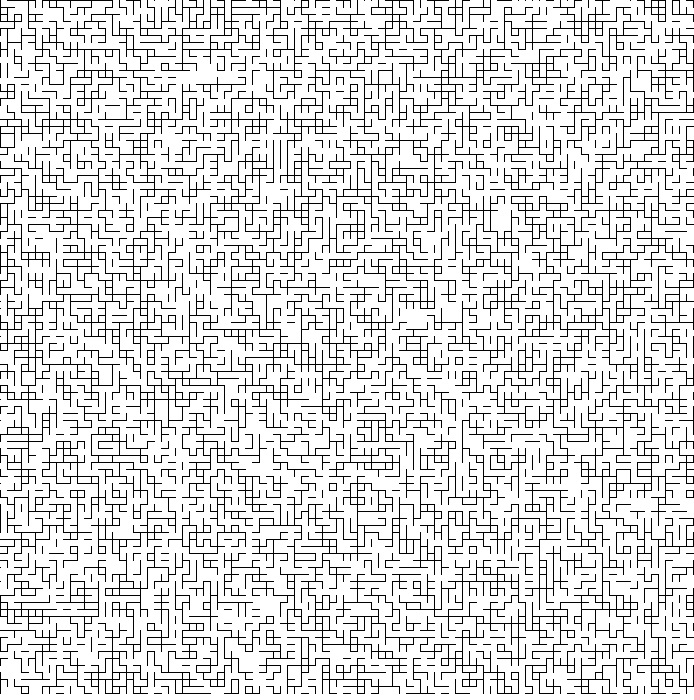
\includegraphics[scale=0.75]{percolation0}
\centering

\caption{Example of a percolation of a $\mathbb{L}^2$ graph (100x100), where p = 0.5}
\end{figure}

\subsubsection{First observations}

We will see some pictures of the simulation rendered by the program with different probabilities. Thus, we can observe how it behaves and have a vague idea of its behavior. \\

\begin{figure}
\begin{tabular}{cc}
  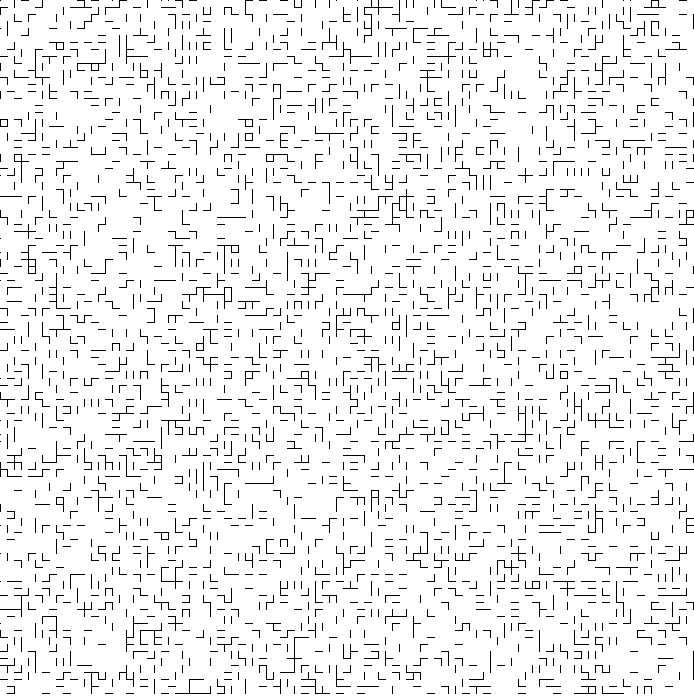
\includegraphics[width=55mm]{perc_20_1} &   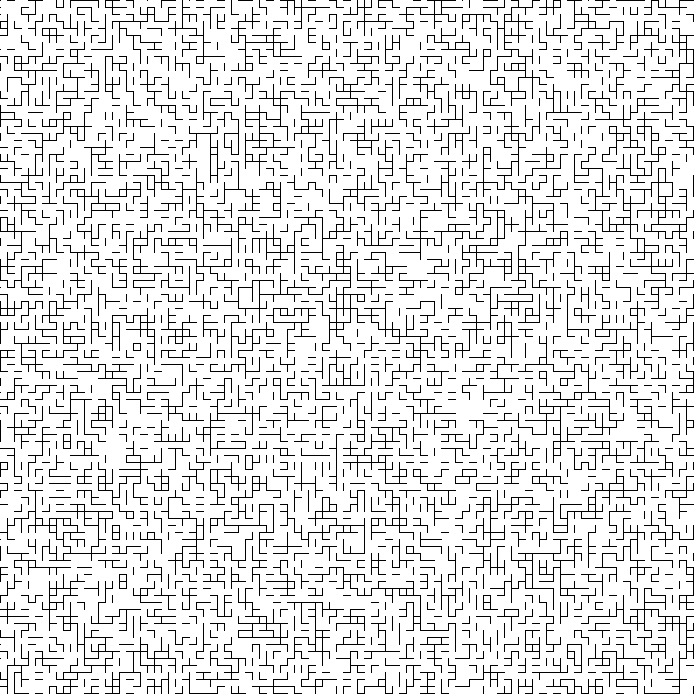
\includegraphics[width=55mm]{perc_40_1} \\
Figure 1 : p = 0.2, Size = 100x100 & Figure 2 : p = 0.4, Size = 100x100 \\[6pt]
 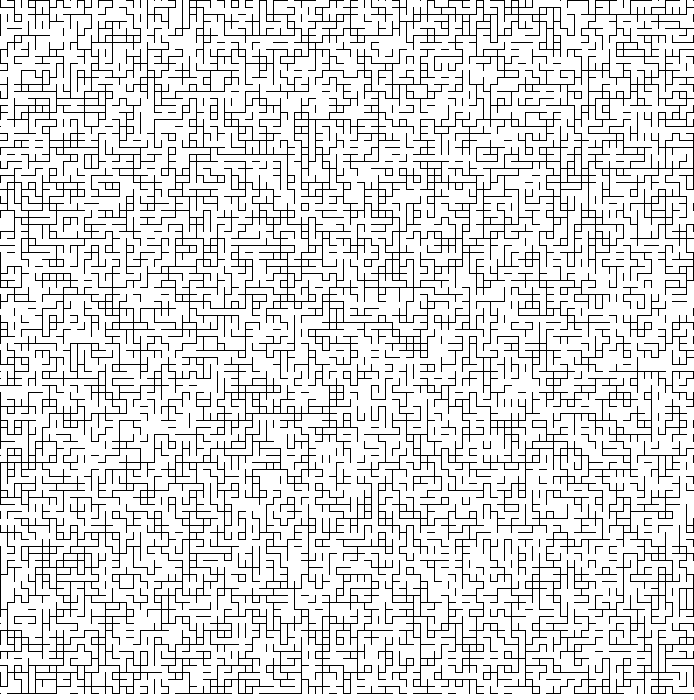
\includegraphics[width=55mm]{perc_50_1} &   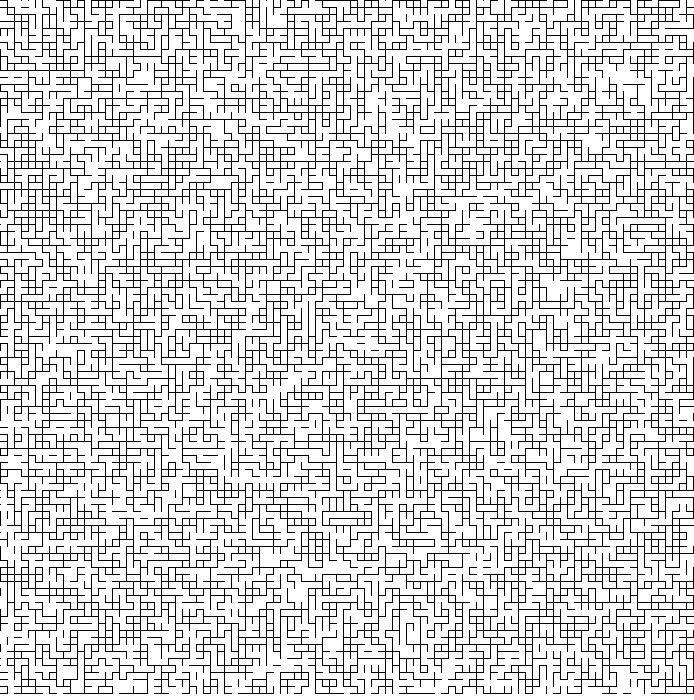
\includegraphics[width=55mm]{perc_60_1} \\
Figure 3 : p = 0.5, Size = 100x100 & Figure 3 : p = 0.6, Size = 100x100 \\[6pt]
\multicolumn{2}{c}{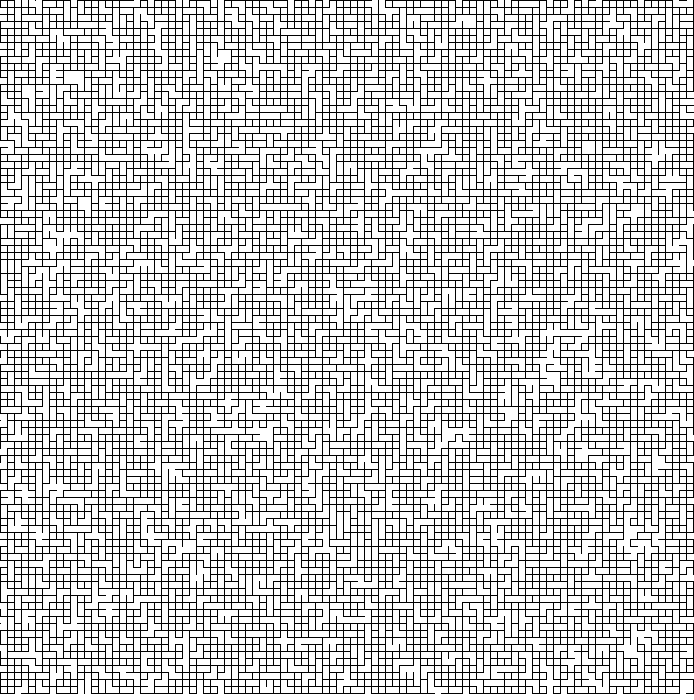
\includegraphics[width=55mm]{perc_80_1} }\\
\multicolumn{2}{c}{Figure 4 : p = 0.8, Size = 100x100}
\end{tabular}
\end{figure}

As we can see the larger is $p$, the more the vertices seems to be connected.
This is all of the point of studying open clusters (rather than connected components as we could imagine)

\subsection{Another point of view}
We had seen the point of view where we choose p and then we percolate. But we can see the other way and define some random uniform variables for each edge between $0$ and $1$, and then discriminate depending on $p$

Let $(X(e), e\in\mathbb{E})$ a family of uniform random variables in $[0,1]$. For $p \in [0,1]$, we say :

$$
\eta_p(e) = \left\{
    \begin{array}{ll}
        0 & \mbox{if $X(e) < p$ (closed)}\\
        1 & \mbox{otherwise (open)}
    \end{array}
\right.
$$

Thus, we can see how it is going. As p is going through $0$ to $1$, the edges are removed going from a complete graph G to a total isolate graph with no edges $(V, \varnothing)$

IMAGES

\subsection{Site percolation}

We have seen the "bond percolation", the percolation of vertices. The other type of percolation is the percolation on vertices, where we remove vertices of a graph with a given probability $p$

As for the "bond percolation", we define $\mathbb{L}^d$, the same way.
But our probability space if different

An edge of G is called open if it is not in G', and closed if it is. 

We consider the following space : $(\Omega, \mathscr{F}, P_p)$ where :
\begin{gather*}
(i) \ \Omega = \prod_{x \in \mathbb{V}}{\{0,1\}} \\
(ii) \ \mathscr{F}=\\
(iii) \ P_p = \prod_{x \in \mathbb{V}}{\mu_{x}}
\end{gather*}

where, $\mu_{x}$ is a Bernoulli measure with a parameter $p\in [0,1]$ for each $x\in\mathbb{V}$. In fact we name configurations the space associated, subset of $\Omega$ where :

$$
\omega(x) = \left\{
    \begin{array}{ll}
        0 & \mbox{if x is closed}\\
        1 & \mbox{if  is open}
    \end{array}
\right.
$$

\subsection{Studying open clusters}
\subsubsection{The Critical phenomenon}
Let study the connected clusters of $\mathbb{L^d}$ depending on $p$. Is there an infinite cluster?
As we saw, we can only restrict ourselves to the origin. Is $C = C(0)$ an infinite cluster?
What we will see is that it exists a critical value $p_c\in [0,1]$ such as: \\

(i) \ if $p < p_c$, then $C$ is almost always an infinite cluster (subcritical phase) \\
(ii) \ if $p > p_c$, then $C$ is almost always not an infinite cluster (supercritical phase) \\
(iii) \ if $p = p_c$, then we are in the critical phase, the most interesting case \\

We can write this as: \\
$$\theta(p) = P_p(|C|=\infty)$$
$$
\theta(p) = \left\{
    \begin{array}{ll}
        0 & \mbox{if $p < p_c$}\\
        1 & \mbox{if $p > p_c$}
    \end{array}
\right.
$$
Where the critical probability p is equal to:
$$p_c = sup\{p \ | \ \theta(p)=0\}$$ \\

\subsubsection{Trivial case of d = 1}

Let's study $\mathbb{L}^1$. We know for sure that if $p < 1$, then almost certainly there will be a closed edge to left of the origin, and to the right. Thus, it will always never have an infinite cluster if $p < 1$. If $p = 1$, it will always have an infinite cluster. \\

\begin{figure}[ht]
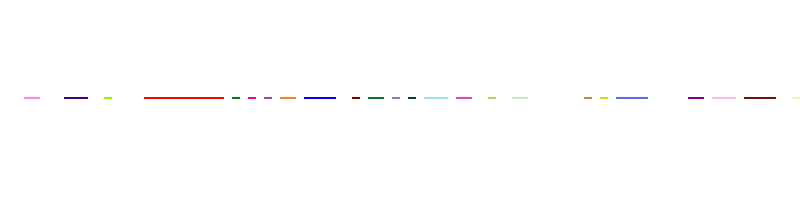
\includegraphics[scale=0.5]{percolationL1}
\centering

\caption{Example of a percolation of a $\mathbb{L}^1$ graph, size = 100, p = 0.5}
\end{figure}

\subsubsection{Case of $d \geq 2$}

To prove we have a critical phenomenon - which means $0 < p_c(d) < 1$, we could restrict ourselves to $d = 2$, and then by induction, deduce it is true for all $d \geq 2$

PROOF

Induction proof :

Base case : True for $d = 2$\\
Induction step :\\

If $0 < p_c(d) < 1$ then,
We know that $\mathbb{L}^(d+1)$ contains $\mathbb{L}^(d)$, because we could fix one coordinate to $0$, and have a subset of dimension $d$ which implies :

$$p_c(d + 1) \leq p_c(d) \forall d \geq 1$$
...

Let's study $\mathbb{L}^d$ for $d \geq 2$.
We have:
$$\Phi(p)=P_p(|C|=\infty)$$
the probability that there exists an infinite cluster. We have :
$$
\Phi(p) = \left\{
    \begin{array}{ll}
        0 & \mbox{if $\theta(p)=0$}\\
        1 & \mbox{if $p > p_c$}
    \end{array}
\right.
$$
It can be translated as the fact that there is almost certainly an infinite cluster if the probability that there is an infinite cluster at the origin is not zero, and is almost impossible otherwise. It shows how studying at a given vertex (here the origin) is equivalent to study for any vertex (which can be far more difficult). It is proven by using the zero-one law which states that if an event, here "the graph contains an infinite cluster" is not dependant upon the states of any finite collection of edges. So, the probability $\Phi(p)$ is equal to $0$ or $1$.

We have two cases ;
If $\theta(p)=0$, the distribution of probability being the same everywhere, $\Phi(p)$ should be equal to $0$.
If it is not zero, then it means $\Phi(p)$ is greater than zero, and it is then $1$.

So the critical phenomenon being proved for the origin, we deduce that there is a probability $p_c$, where under this probability, there is almost never an infinite cluster, if below there is almost always an infinite cluster.

We can see the same images presented in 1.1.1 but with the open clusters colored in order to visualize the phenomenon. The larger open cluster is colored in red so it is easily viewable. (?)

\begin{figure}
\begin{tabular}{cc}
  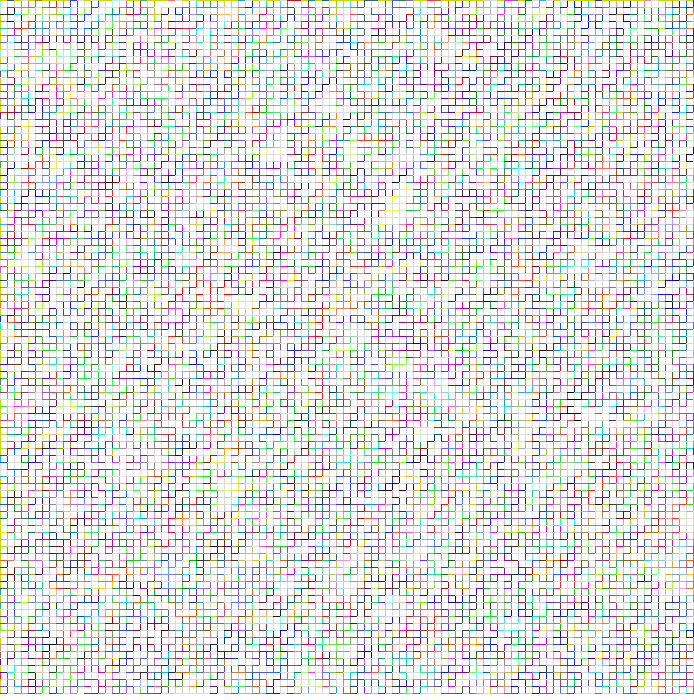
\includegraphics[width=55mm]{perc_20_2} &   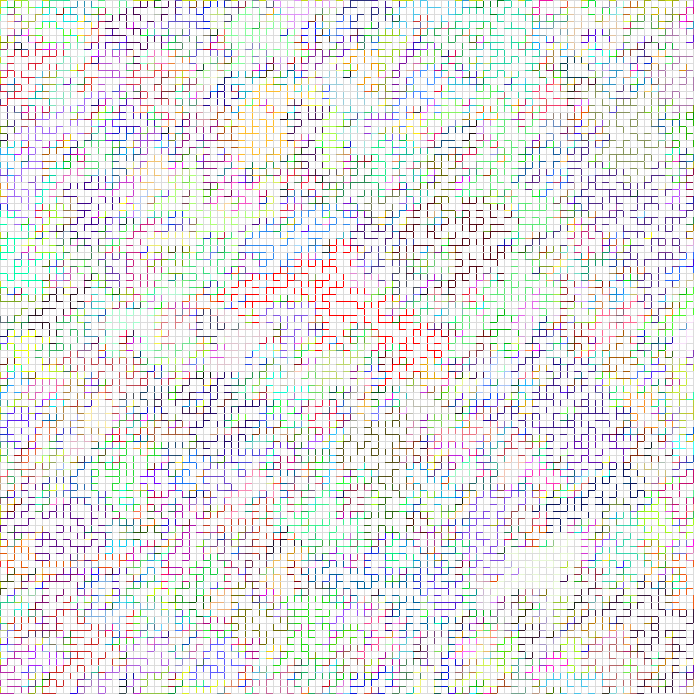
\includegraphics[width=55mm]{perc_40_2} \\
Figure 1 : p = 0.2, Size = 100x100 & Figure 2 : p = 0.4, Size = 100x100 \\[6pt]
 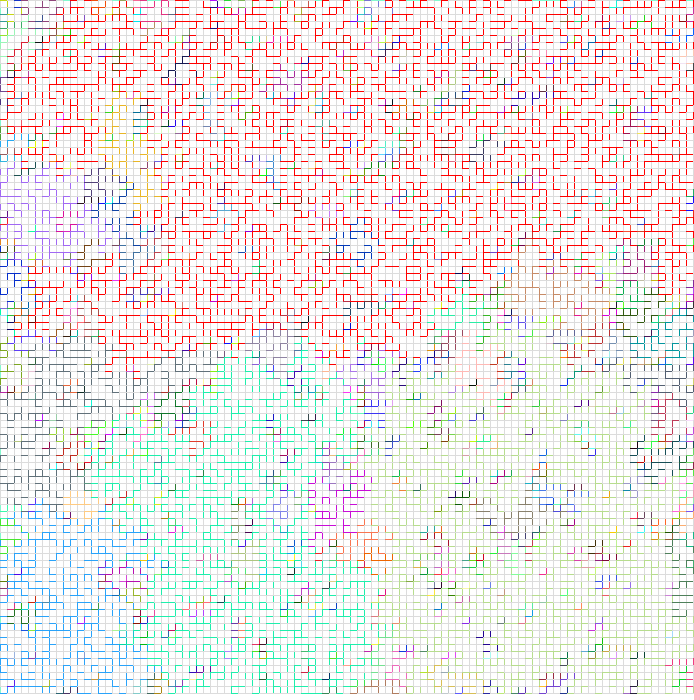
\includegraphics[width=
 55mm]{perc_50_2} &   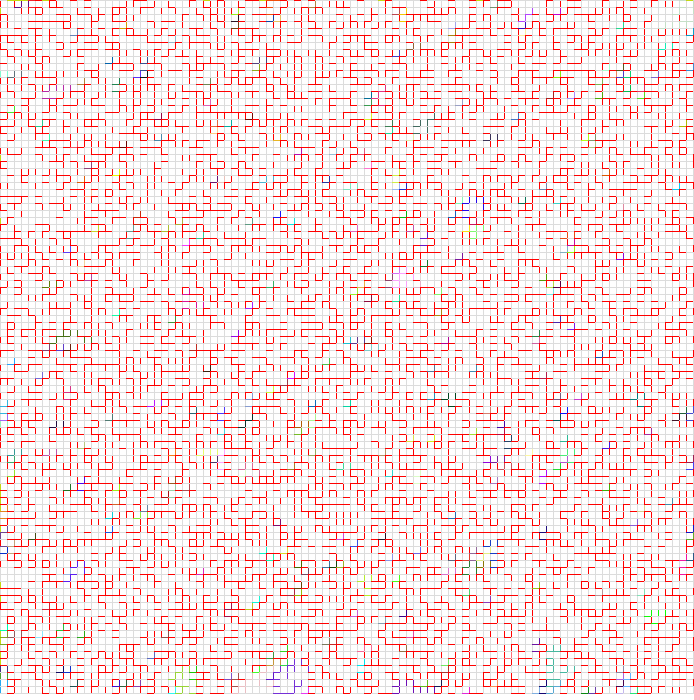
\includegraphics[width=55mm]{perc_60_2} \\
Figure 3 : p = 0.5, Size = 100x100 & Figure 3 : p = 0.6, Size = 100x100 \\[6pt]
\multicolumn{2}{c}{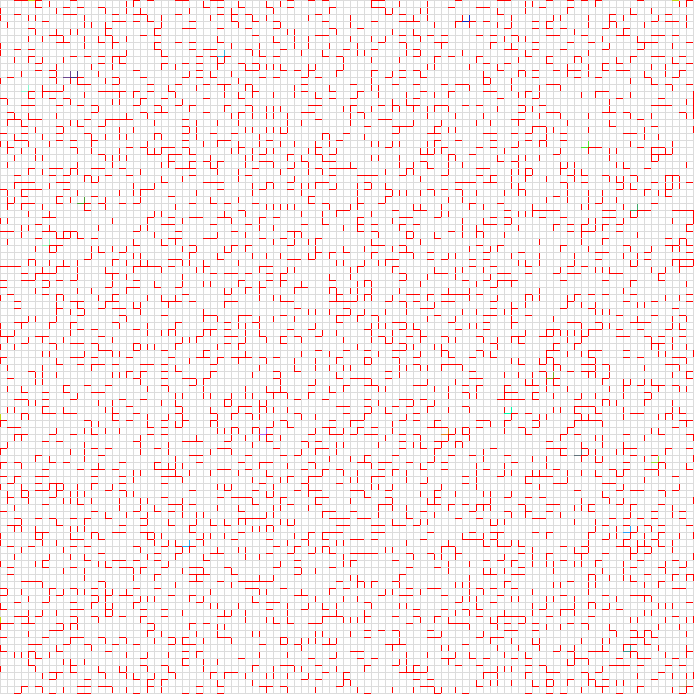
\includegraphics[width=55mm]{perc_80_2} }\\
\multicolumn{2}{c}{Figure 4 : p = 0.8, Size = 100x100}
\end{tabular}
\end{figure}

\subsection{Uniqueness of the infinite cluster}

\subsection{Critical phenomenon for site percolation}

As for bond percolation we observe the same phenomenon. An open cluster $C(x)$ is defined for a vertex $x$ as a connected component of $K(w)$ which is the subset of open vertices.
So we can define our percolation probability $\theta(p) = P_p(|C|=\infty)$ and the critical probability 
$$p_c = sup\{p \ | \ \theta(p) = 0 \}$$

All of our previous demonstration for bond percolation can be converted on site percolation, thus we will not try to repeat what was said before.

\subsubsection{Relation between the two}

Let's $G$ be a graph. \\
$G_c$ is a covering graph of the graph $G$ if and only it is a subgraph of $G$ and if it contains all of the vertices of $G_c$ such as the set of incident edges of the vertices of $G_c$

For $G$, we study the "bond percolation". For $G_c$, we study the "site percolation" by defining this way:\\
A vertex $x$ is open if and only if the corresponding edge is open. (?)
All of the paths of open edges are directly corresponded to a path of open vertices in $G_c$. Studying "site percolation" for $G_c$ is equivalent to study "bond percolation" for $G$.

\subsection{Study of critical probabilities}

Our goal is to find the critical probability for $G = \mathbb{L}^2$, it seems like it is equal to $p_c = 0.5$, but we can be sure if we didn't prove it. \\
There is not always for $p_c$ a clear value, or a clear formula to find but there are some cases where it is true and can only be approached by algorithms.

\subsubsection{Table of other cases for two dimensions lattices}
Here is summarized briefly some cases where the value was found. \\
This part is not very important for the rest of the study and only for general culture.

\begin{figure}
\begin{tabular}{cc}
  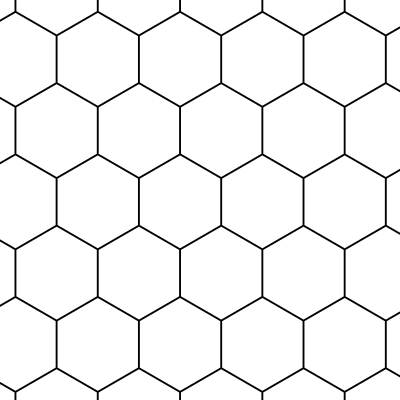
\includegraphics[width=55mm]{hexagonal_lattice} &   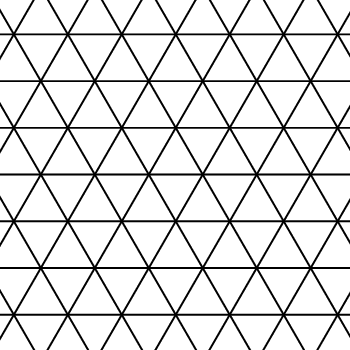
\includegraphics[width=55mm]{triangular_lattice} \\
Figure 1 : Honeycomb lattice, $p_c = 1 - 2 * sin(\frac{\pi}{18})$ & Figure 2 : Triangular, $p_c = 2sin(\frac{\pi}{18})$ \\[6pt]
 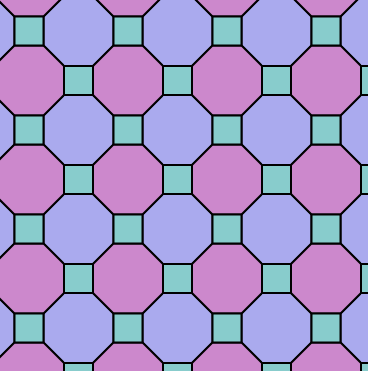
\includegraphics[width=
 55mm]{truncated_square_lattice} &   
\includegraphics[width=55mm]{square_lattice} \\
Figure 3 : $Truncated square$ lattice\\ Equation : $4p_c^3 + 3p_c^4 - 6p_c^5 - 2p_c^6 = 1$ & Figure 4 : Square lattice, $p_c = \frac{1}{2}$\\[2pt]
\end{tabular}
\end{figure}

\subsubsection{Duality and bond percolation}

An important concept for calculating $p_c$ for a given planar graph, is to study its dual graph (where faces are transformed into vertices and they are connected by an edge when the faces have one edge in common).\\
We can immediately see that the dual graph of $L^2$ is indeed himself. So if we can find a relation between the critical probability for a given lattice and the critical probability for its dual graph, we might prove that $p_c = 0.5$.
And there is one :\\

For all planar lattice $\mathscr{L}$, if $\mathscr{L}_d$ is its dual lattice, then :

$$p_c(\mathscr{L}) + p_c(\mathscr{L}_d) = 1$$
So we can see how we will prove that $p_c = 0.5$ for the square lattice, because :

$$p_c(\mathscr{L}) = p_c(\mathscr{L}_d) = \frac{1}{2}$$

which is the same as,

$$ p > p_c(\mathscr{L}) \Longleftrightarrow 1 - p < p_c(\mathscr{L}_d)$$

Because if $p > p_c(\mathscr{L})$, then almost surely, $\mathscr{L}$ has an infinite open cluster. Because it is unique and extends through space, $\mathscr{L}_d$ can't have an infinite closed cluster. Which means that $1 - p < p_c{\mathscr{L}_d}$ \\

Also, thus for other types of lattices we can link graphs with there duals :
The dual of a triangular lattice is an hexagonal lattice for instance.
...

\subsubsection{Site percolation and matching}


\begin{figure}[ht]
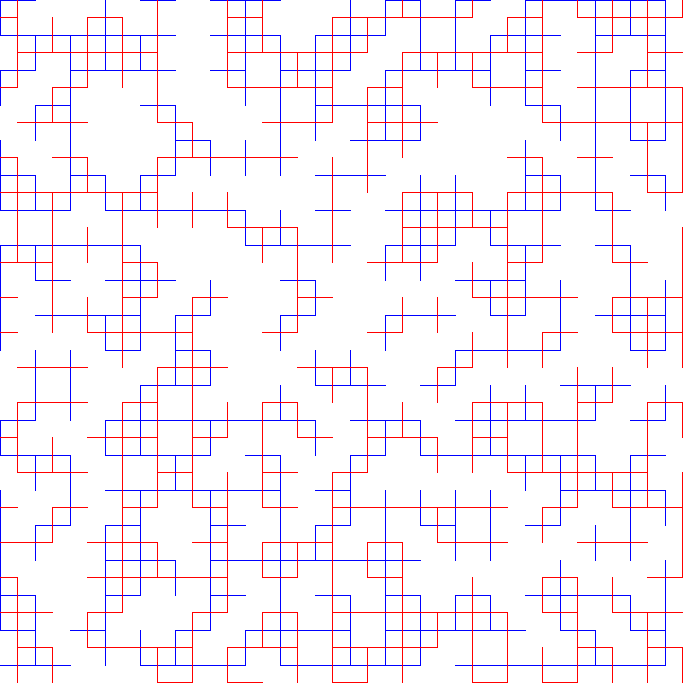
\includegraphics[scale=0.5]{dual}
\centering

\caption{A subgraph of $\mathbb{L}^2$ (in blue) and its dual (in red), p = 0.5, Size = 20x20}
\end{figure}

\subsection{Appendix : Some equalities and inequalities}

First we define $p_c^{bond}(G)$ as the critical probability for $G$ for bond percolation, and $p_c{site}(G)$ as the critical probability for $G_c$ for site percolation. \\
It is clear that : $p_c{bond}(G) = p_c{site}(G)$

\subsection{Some useful inequalities}
Let $(\Omega, \mathscr{F})$ be our space couple. \\
Here we don't study only $\mathbb{L}^d$ but a general probability space. \\

\subsubsection{Partial order on $(\Omega, \mathscr{F})$}
We have $\forall \omega, \omega' \in \mathscr{F}, \omega \leq \omega' \Longleftrightarrow \omega(e) \leq \omega'(e) \forall e \in \mathbb{E})$
This define a partial order on $(\Omega, \mathscr{F})$ which will be very useful to discover inequalities.\\
Here in the special case of $\mathbb{L}^d$, we easily see for $K(\Omega)$ being the set of open edges of $\mathbb{L}^d$ of the lattice that :
$$\omega \leq \omega' \Longleftrightarrow K(\omega) \subseteq K(\omega')$$

\subsubsection{Increasing function and events}
Definition: Increasing function

We say that $\Psi(p)$ is an increasing function of p if :
In a measurable pair, $(\Omega, \mathscr{F})$, for $w, w' \in \mathscr{F}$
$$w \leq w' \implies \Psi(w) \leq \Psi(w')$$

And $\Psi(p)$ is decreasing if $-N$ is increasing \\

\subsubsection{First inequalities}
First inequalities :
If $N$ is an increasing random variable on $(\Omega, \mathscr{F})$, then : \\
If $p_1 \leq p_2$ and $\mathbb{E}_{p_1}(N) < \infty$ and $\mathbb{E}_{p_2}(N) < \infty$ then $\mathbb{E}_{p_1}(N) \leq \mathbb{E}_{p_2}(N)$ \\

If $A$ is an increasing event in $\mathscr{F}$ then
(ii) If $p_1 \leq p_2$ then $P_{p_1}(N) \leq P_{p_2}(N)$ \\

\subsubsection{Other inequalities}

FKG inequalities : \\

If $X$ and $Y$ are increasing (decreasing) random variables and $\mathbb{E}_p{(X^2)} < \infty$ and $\mathbb{E}_p{(Y^2)} < \infty$, then \\
(iii)
$$\mathbb{E}_p(XY) \geq \mathbb{E}_p(X)\mathbb{E}_p(Y)$$

If $A$ and $B$ are increasing (decreasing) events, then \\
(iv)
$$\mathbb{P}_p(A \cap B) \geq \mathbb{P}_p(A)\mathbb{P}_p(B)$$

If  $X$ is increasing and $Y$ is decreasing random variables and $\mathbb{E}_p{(X^2)} < \infty$ and $\mathbb{E}_p{(Y^2)} < \infty$, then \\
(v)
$$\mathbb{E}_p(XY) \leq \mathbb{E}_p(X)\mathbb{E}_p(Y)$$

If $A$ is increasing and $B$ is decreasing (or the other way) events, then \\
(vi)
$$\mathbb{P}_p(A \cap B) \leq \mathbb{P}_p(A)\mathbb{P}_p(B)$$

\subsubsection{Application of these inequalities}

If for $x \in V$, we have $\theta(p, x)$, the probability that x is in an infinite open cluster, then we have :
$p_c(x)=sup\{p \ | \ \theta(p,x) = 0\}$

By the precedent inequality, we have

$$\theta(p, x) \geq P_p(\{x \longleftrightarrow y \} \cap \{y \longleftrightarrow \infty \}) \geq P_p(x \longleftrightarrow y)\theta(p, y)$$

when $p_c(x) \leq p_c(y)$ (?)

We deduce the following theorem :

Let G be an infinite connected graph with a countable number of edges. The value of the bond critical probability $p_c^{bond}(x)$ and the site critical probability $p_c^{site}(x)$ are independent of the choice of the initial vertex $x$ (?)

\subsubsection{BK and Russo inequalities}

BK inequality :\\

If $A$ and $B$ are increasing events in $\mathscr{G}$ then :
$$P(A \circ B) \leq P(A)P(B)$$

BK inequality application on bond percolation for $\mathbb{L}^d$ :\\
Let $A$ and $B$ two increasing events on $\mathbb{L}^d$, then :

$$P_p(A \circ B) \leq P_p(A)P_p(B)$$

\end{document}
